\documentclass[ignorenonframetext,]{beamer}
\setbeamertemplate{caption}[numbered]
\setbeamertemplate{caption label separator}{: }
\setbeamercolor{caption name}{fg=normal text.fg}
\beamertemplatenavigationsymbolsempty
\usepackage{lmodern}
\usepackage{amssymb,amsmath}
\usepackage{ifxetex,ifluatex}
\usepackage{fixltx2e} % provides \textsubscript
\ifnum 0\ifxetex 1\fi\ifluatex 1\fi=0 % if pdftex
  \usepackage[T1]{fontenc}
  \usepackage[utf8]{inputenc}
\else % if luatex or xelatex
  \ifxetex
    \usepackage{mathspec}
  \else
    \usepackage{fontspec}
  \fi
  \defaultfontfeatures{Ligatures=TeX,Scale=MatchLowercase}
\fi
% use upquote if available, for straight quotes in verbatim environments
\IfFileExists{upquote.sty}{\usepackage{upquote}}{}
% use microtype if available
\IfFileExists{microtype.sty}{%
\usepackage{microtype}
\UseMicrotypeSet[protrusion]{basicmath} % disable protrusion for tt fonts
}{}
\newif\ifbibliography
\hypersetup{
            pdftitle={Electricity Load Prediction in Texas},
            pdfauthor={Alan Yu, Justin Mei},
            pdfborder={0 0 0},
            breaklinks=true}
\urlstyle{same}  % don't use monospace font for urls
\usepackage{graphicx,grffile}
\makeatletter
\def\maxwidth{\ifdim\Gin@nat@width>\linewidth\linewidth\else\Gin@nat@width\fi}
\def\maxheight{\ifdim\Gin@nat@height>\textheight0.8\textheight\else\Gin@nat@height\fi}
\makeatother
% Scale images if necessary, so that they will not overflow the page
% margins by default, and it is still possible to overwrite the defaults
% using explicit options in \includegraphics[width, height, ...]{}
\setkeys{Gin}{width=\maxwidth,height=\maxheight,keepaspectratio}

% Prevent slide breaks in the middle of a paragraph:
\widowpenalties 1 10000
\raggedbottom

\AtBeginPart{
  \let\insertpartnumber\relax
  \let\partname\relax
  \frame{\partpage}
}
\AtBeginSection{
  \ifbibliography
  \else
    \let\insertsectionnumber\relax
    \let\sectionname\relax
    \frame{\sectionpage}
  \fi
}
\AtBeginSubsection{
  \let\insertsubsectionnumber\relax
  \let\subsectionname\relax
  \frame{\subsectionpage}
}

\setlength{\parindent}{0pt}
\setlength{\parskip}{6pt plus 2pt minus 1pt}
\setlength{\emergencystretch}{3em}  % prevent overfull lines
\providecommand{\tightlist}{%
  \setlength{\itemsep}{0pt}\setlength{\parskip}{0pt}}
\setcounter{secnumdepth}{0}

\title{Electricity Load Prediction in Texas}
\author{Alan Yu, Justin Mei}
\date{4/30/2019}

\begin{document}
\frame{\titlepage}

\begin{frame}[fragile]{Introduction/Background}

\begin{itemize}
\tightlist
\item
  Data is from Electric Reliability Council of Texas (ERCOT)
\item
  Manages the flow of electricity power and represents over 90\% of the
  state's electric load
\item
  Our focus is to predict the next 24 hour load based on past historical
  data
\end{itemize}

\begin{verbatim}
## Warning: package 'png' was built under R version 3.5.2
\end{verbatim}

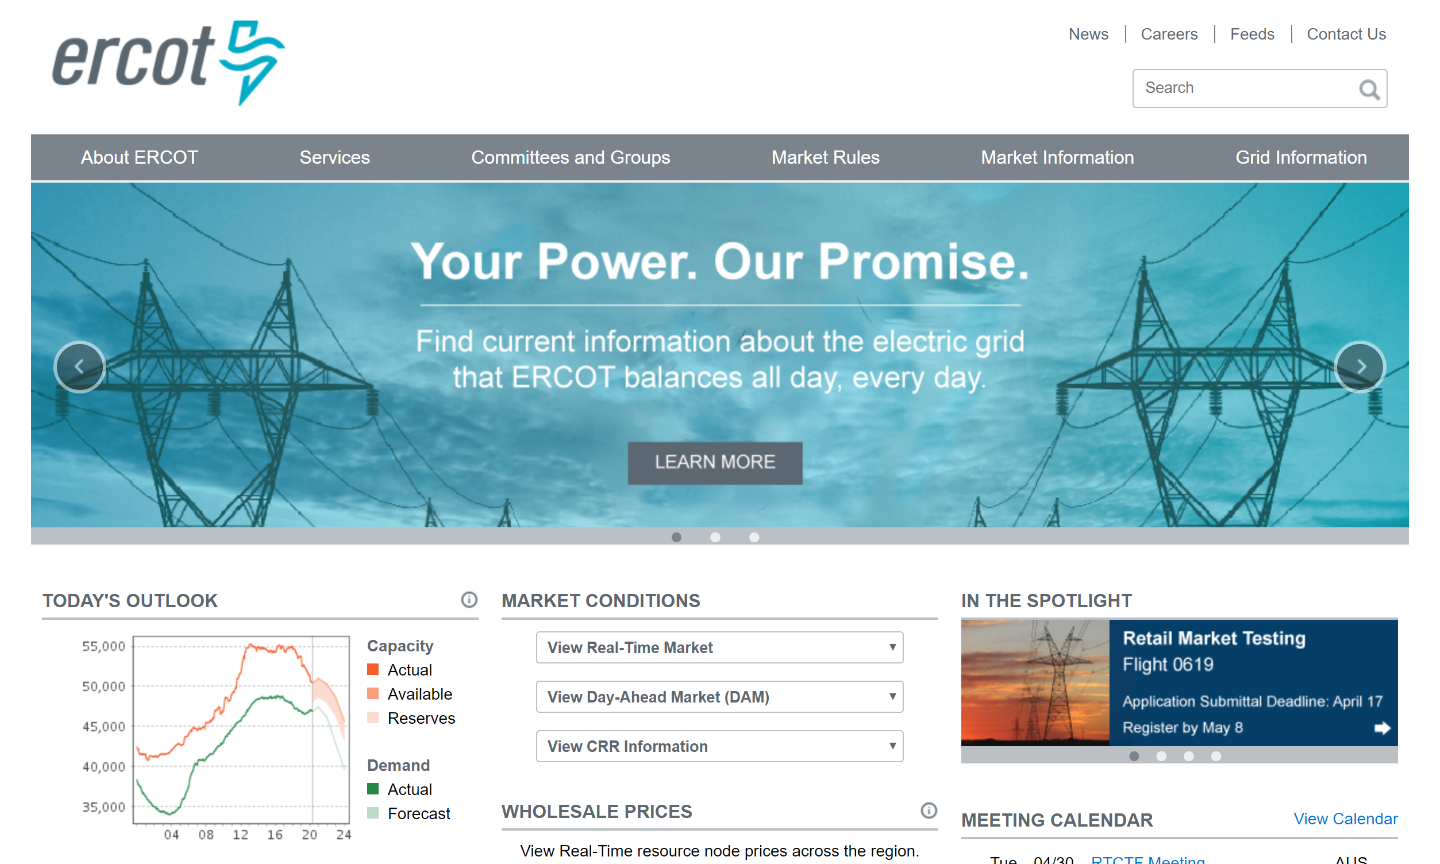
\includegraphics{Final_Presentation_files/figure-beamer/unnamed-chunk-1-1.pdf}
- GOAL: Predict the next 24 hour load using past history of demands

\end{frame}

\begin{frame}{Data Exploration}

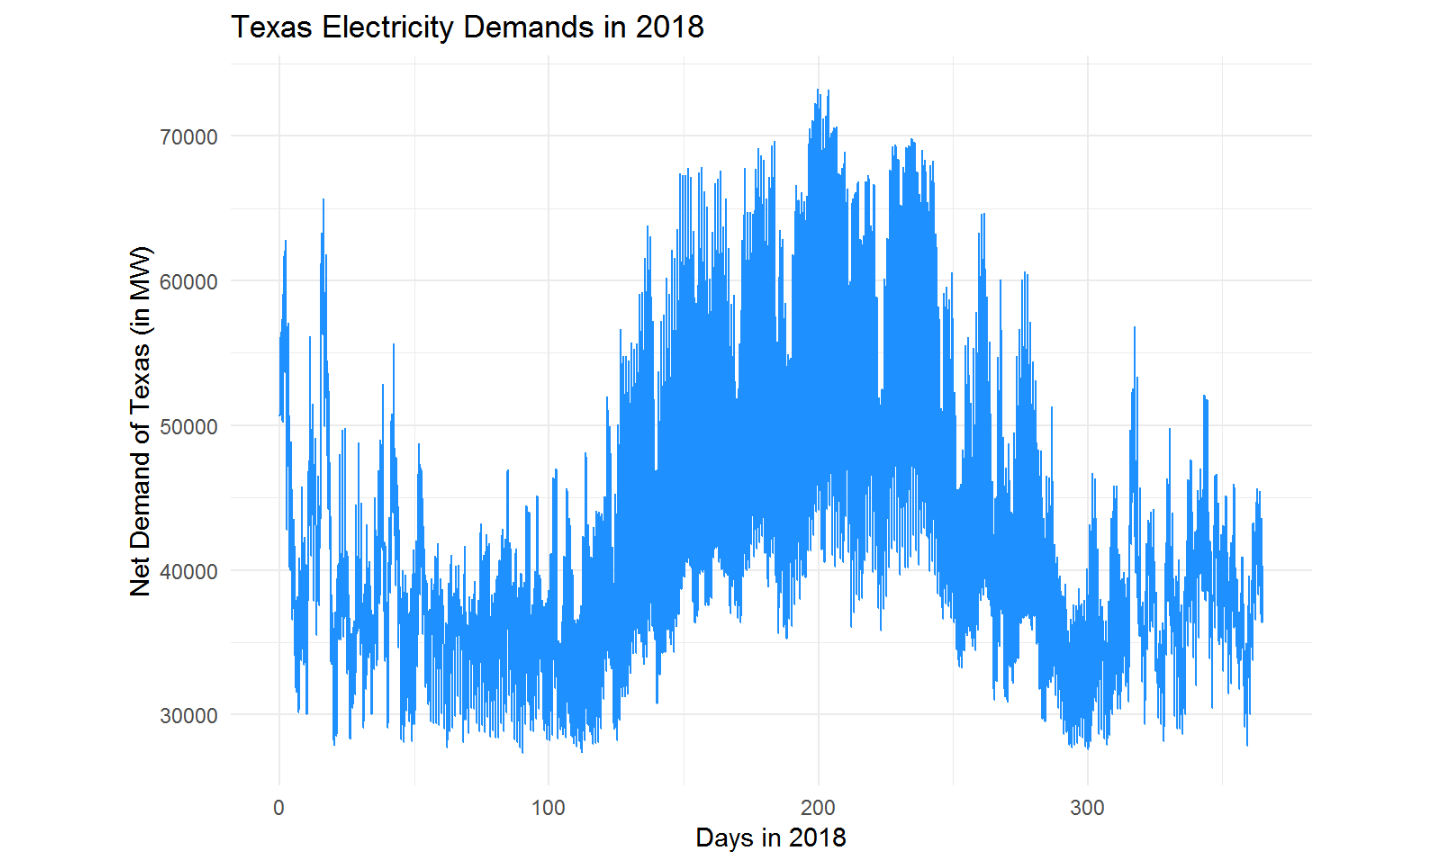
\includegraphics{Final_Presentation_files/figure-beamer/unnamed-chunk-2-1.pdf}

A peak around the summer time; noticeable trend

Texas has a similar climate to Illinois. High energy usage in summers
and winters.

\end{frame}

\begin{frame}{Load in Spring(March) vs Load in Summer(July)}

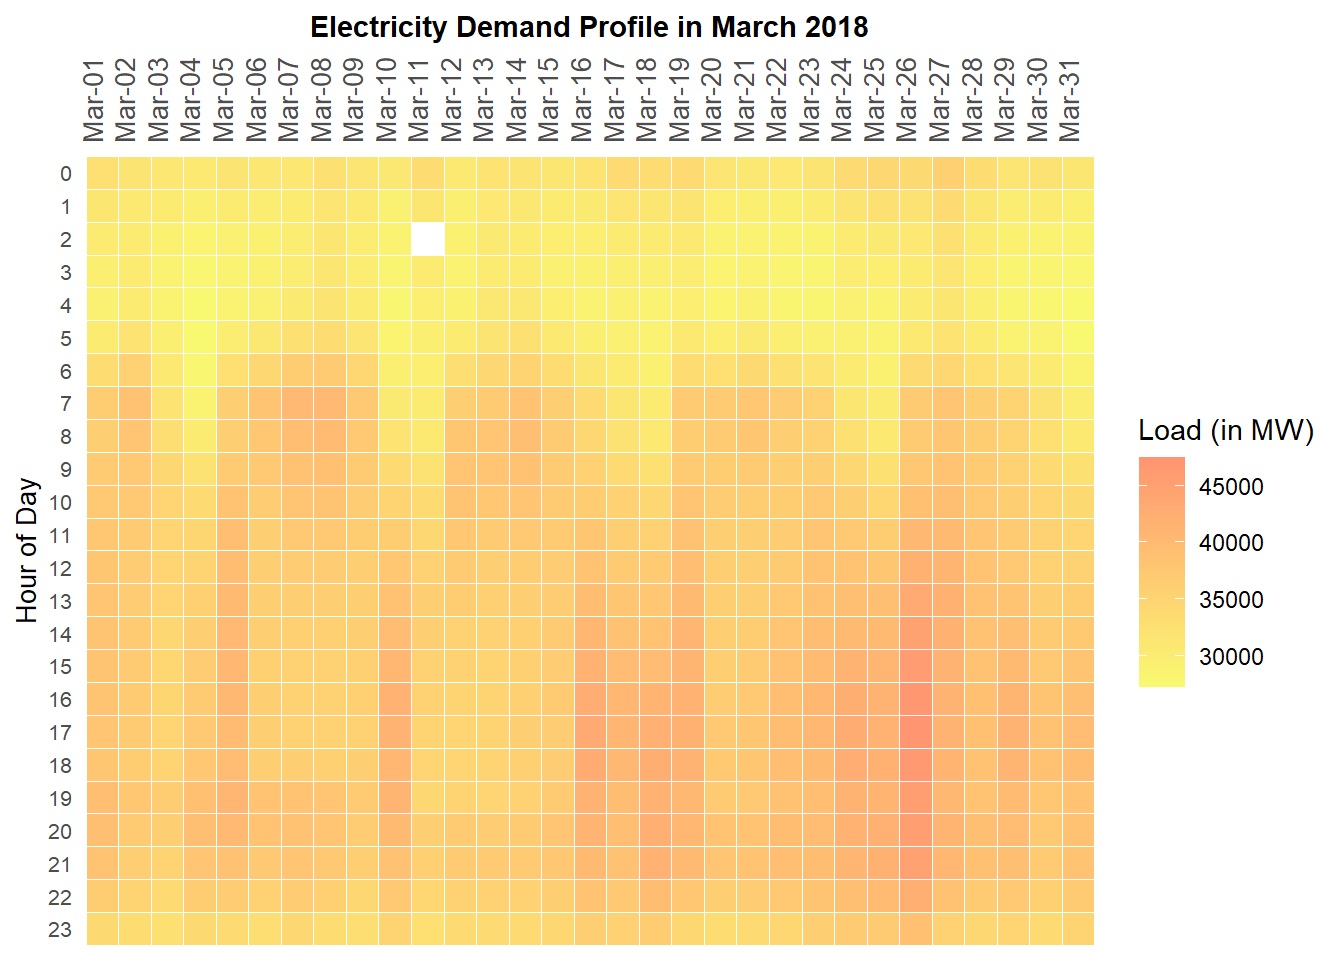
\includegraphics[width=0.49000\textwidth]{README-March HeatMap-1.png}
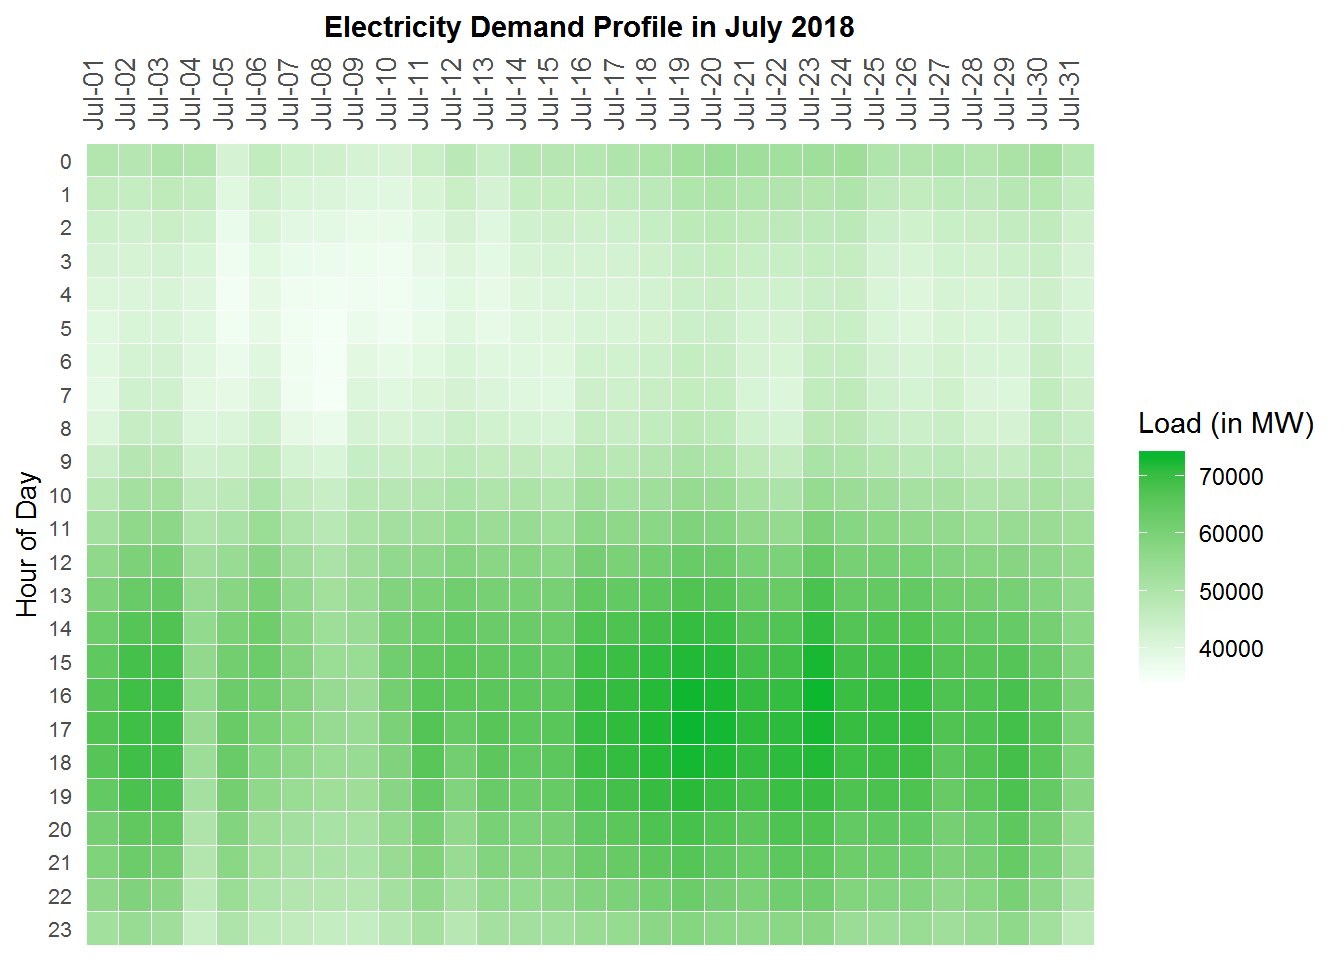
\includegraphics[width=0.49000\textwidth]{README-July HeatMap-1.png}

Relatively low energy consumption in the mornings, high in the
afternoons and evenings

Very hot in the summer = a lot air conditioners in use, everyday looks
very similar

\end{frame}

\begin{frame}{Prediction Strategy}

\begin{itemize}
\item
  3 features: Load at hour t from the exact moment 7 days, 2 days and 1
  day ago
\item
  Split data in train (284 days) and test (72 days) set
\item
  Predict Demand at Hour t, \(t \in \left \{0,1,2...23 \right \}\)
  \[ Demand_{t}=\beta_{0}+\beta_{1} \text {7days ago}_{t}+\beta_{2} \text {2days ago }_{t}+\beta_{3} \text { 1day ago}_{t} + \epsilon\]
\item
  In total: 24 regression models for each hour of a day
\end{itemize}

\end{frame}

\begin{frame}{Results \& Room for Improvement}

Testing Acc: 81\% ; Could be better if used non-linear methods (NN,
ARIMA)
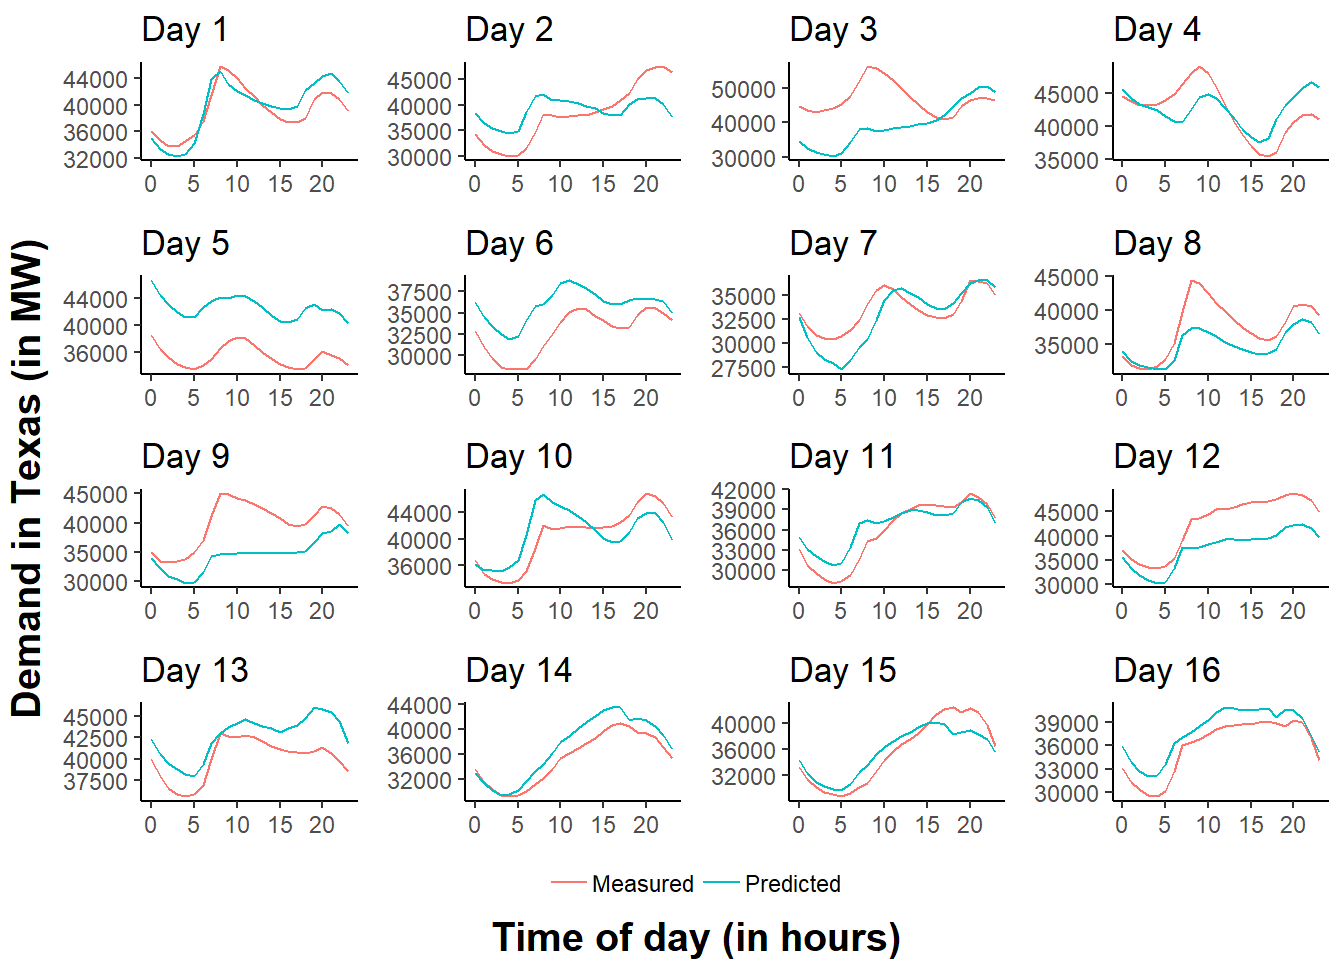
\includegraphics[width=0.74000\textwidth]{README-unnamed-chunk-8-1.png}

\end{frame}

\end{document}
